\chapter{Informaci�n de campo.}

\section{Recorrido de campo}

El recorrido de campo se realiz\'o entre los d\'ias 22 y 24 de Noviembre de 2017. La zona recorrida se tuvo como prop\'osito inspeccionar aquellos lugares que mostraron menor factor de seguridad en las pruebas preliminares y apreciar el estado de las unidades geol\'ogicas que muestra la cartograf\'ia estudiada. 

En campo se pudo corroborar la consistencia de la unidad geol\'ogica predominante Ksaau (limolita), dicho material se pudo apreciar en todo el recorrido, con leve variaci\'on en su grado de meteorizaci\'on, principalmente en zonas de abundante vegetaci\'on. La morfolog\'ia abrupta de las laderas permiti\'o apreciar abundantes cicatrices de anteriores desprendimientos de material, principalmente en sectores de alta pendiente y en el trazado de la carretera el Carmen - Choc\'o.

Se realizaron 2 estaciones, en cada una de las cuales se realiz\'o la respectiva toma de muestra, siendo la primera de ellas la que m\'as informaci\'on proveer\'ia en los posteriores ensayos de laboratorio. Para la toma de muestra se tuvo la precauci\'on de seleccionar un lugar que no presentase retrabajamiento del material y en el cual se pudiese observar que el suelo presentase unas condiciones representativas del material observado durante los recorridos realizados.
Las muestras tomadas en la segunda estaci\'on se tomaron a una profundidad m\'a s somera con la intenci\'on de, posteriormente, poder obtener los par\'a metros de resistencia de instancias m\'a s avanzadas de meteorizaci\'on de la limonita. Esto dado que las cicatrices de movimientos en masa observadas aparentaban que aquellos eventos ocurridos se dieron hace un tiempo considerable(a juzgar por el crecimiento nueva cobertura vegetal) no contaron con profundidades considerables de su respectiva superficie de falla. Asimismo, el testimonio obtenido de una habitante del lugar, corrobora que no son frecuentes movimientos que comprendan altos vol\'umenes de material, habiendo ocurrido el \'ultimo aproximadamente 5 a�os antes de la visita de campo.

La estaci�n 1 se realiz� en las coordenadas \textbf{5.8712778,-76.0848778}, mientras que la estaci�n 2 se realiz� en las las coordenadas \textbf{5.8612472,-76.0927833} :

\textbf{Muestras recolectadas}



De la estaci�n 1 se obtuvo:
\begin{itemize}
  \item Muestra al interior de 4 tubos PVC de 2 pulgadas de di�metro y aproximadamente 15 cm de alto.
  \item 1 Bloque de muestra inalterada  de aproximadamente 40cm x 40cm x 30cm.
  \item 200gr de muestra alterada.
\end{itemize}

De la estaci�n 2 se obtuvo:
\begin{itemize}
  \item Muestra al interior de 3 tubos PVC de 2 pulgadas de di�metro y aproximadamente 15 cm de alto.
\end{itemize}

El registro fotogr�fico de ambas estaciones y del recorrido realizado se incluye a manera de anexos.


\section{Ensayos de laboratorio.}

Las muestras recolectadas fueron analizadas en el laboratorio de suelos de a universidad nacional sede Medell�n.
Como resultado de los ensayos se pudo determinar una humedad natural del 20.89\%.
La gravedad espec�fica de los solidos, seg�n el procedimiento descrito en la norma ASTM C-127. fue de 2.53.
Con estos valores se procedi� a realizar los ensayos de corte directo seg�n la norma ASTM D'380. Se decidi� realizar los ensayos bajo condiciones de suelo saturado, con el prop�sito de obtener par�metros correspondientes a eventos de alta precipitaci�n que puedan presentarse en la zona de trabajo.
Los par�metros de resistencia obtenidos son �ngulo de fricci�n = 40, cohesion = 29 kPa. Las hojas de calculo de estos ensayos se adjuntan como anexos al presente trabajo.

\textbf{Scoops3D.}
Tomando los resultados de laboratorio expuestos anteriormente se procedi� a ingresar los valores correspondientes a angulo de fricci�n, cohesi�n y gravedad especifica en Scoops3D. Se mantuvo la configuraci�n de caja de b�squeda descrita en la subseccion XX, el DEM de la subseccion XX.


\begin{figure}[H]
\centering
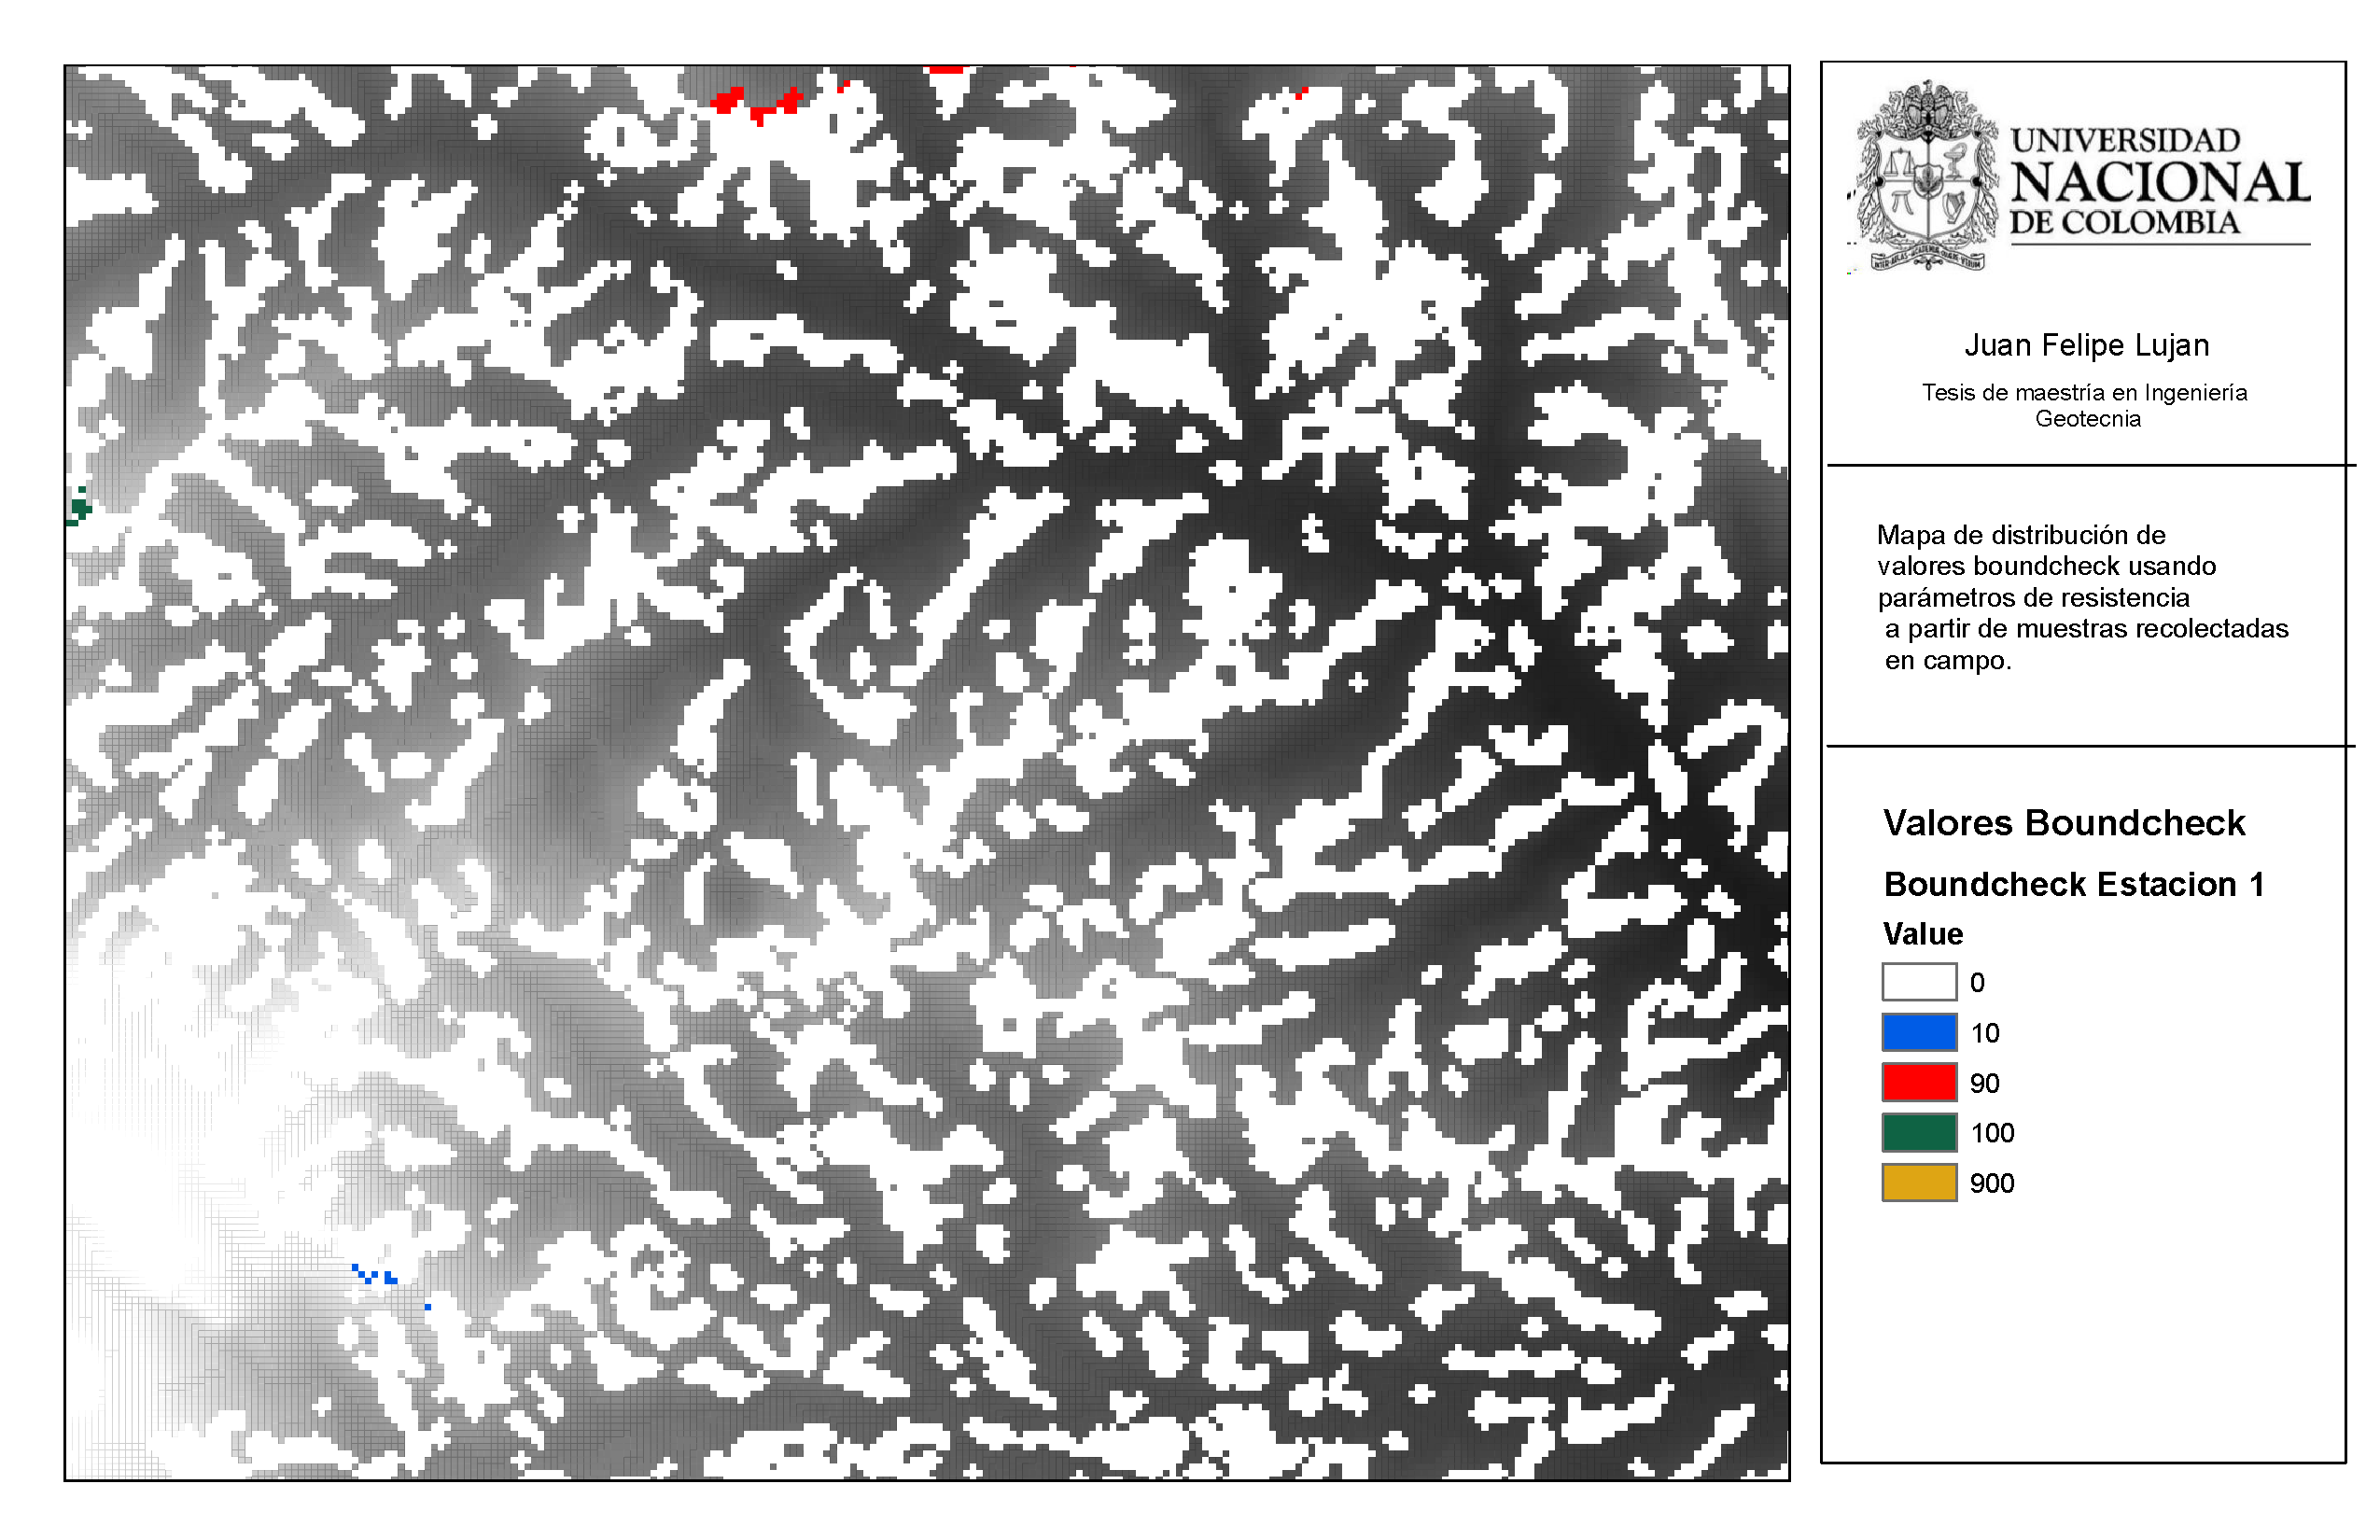
\includegraphics[scale=0.3]{img/boundcheckCampo.pdf}
\caption{Visualizacion del archivo de salida Boundcheck. Fuente: Elaboraci�n propia.}
\label{fig:dem usado}
\end{figure}



Se puede apreciar en el archivo de salida boundcheck que la caja de busqueda propuesta en las pruebas preliminares es aplicable  los datos obtenidos de las muestras recolectadas en campo. Dicho comportamento era esperado debido a la abundancia de pendientes pronunciadas en esta zona del municipio de Ciudad Bolivar. 


Los p�xeles marcados con color azul en el sector suroccidental de la zona de trabajo indican que la extension de la caja de busqueda hacia el extremo sur fue una limitante para aplicar el m�todo bishop (centro de la superficie de falla por fuera de la caja de busqueda, en direccion sur) lo mismo ocurre con los pixeles marcados de color rojo hacia el extremo norte de la zona de trabajo (centro de la superficie de falla por fuera de la caja de busqueda, en direccion norte)

Sin embargo, dado que la cuenta de p�xeles donde se presenta dicho comportamiento es de 89 sobre un total de 28057, se puede decir que la caja de busqueda usada es aplicable en un 99.996\% a la zona de trabajo.
Para aumentar la cobertura ser�a necesario realizar pruebas en equipos de computo con mayores capacidades de computo a las descritas en el capitulo 5.


\begin{figure}[H]
\centering
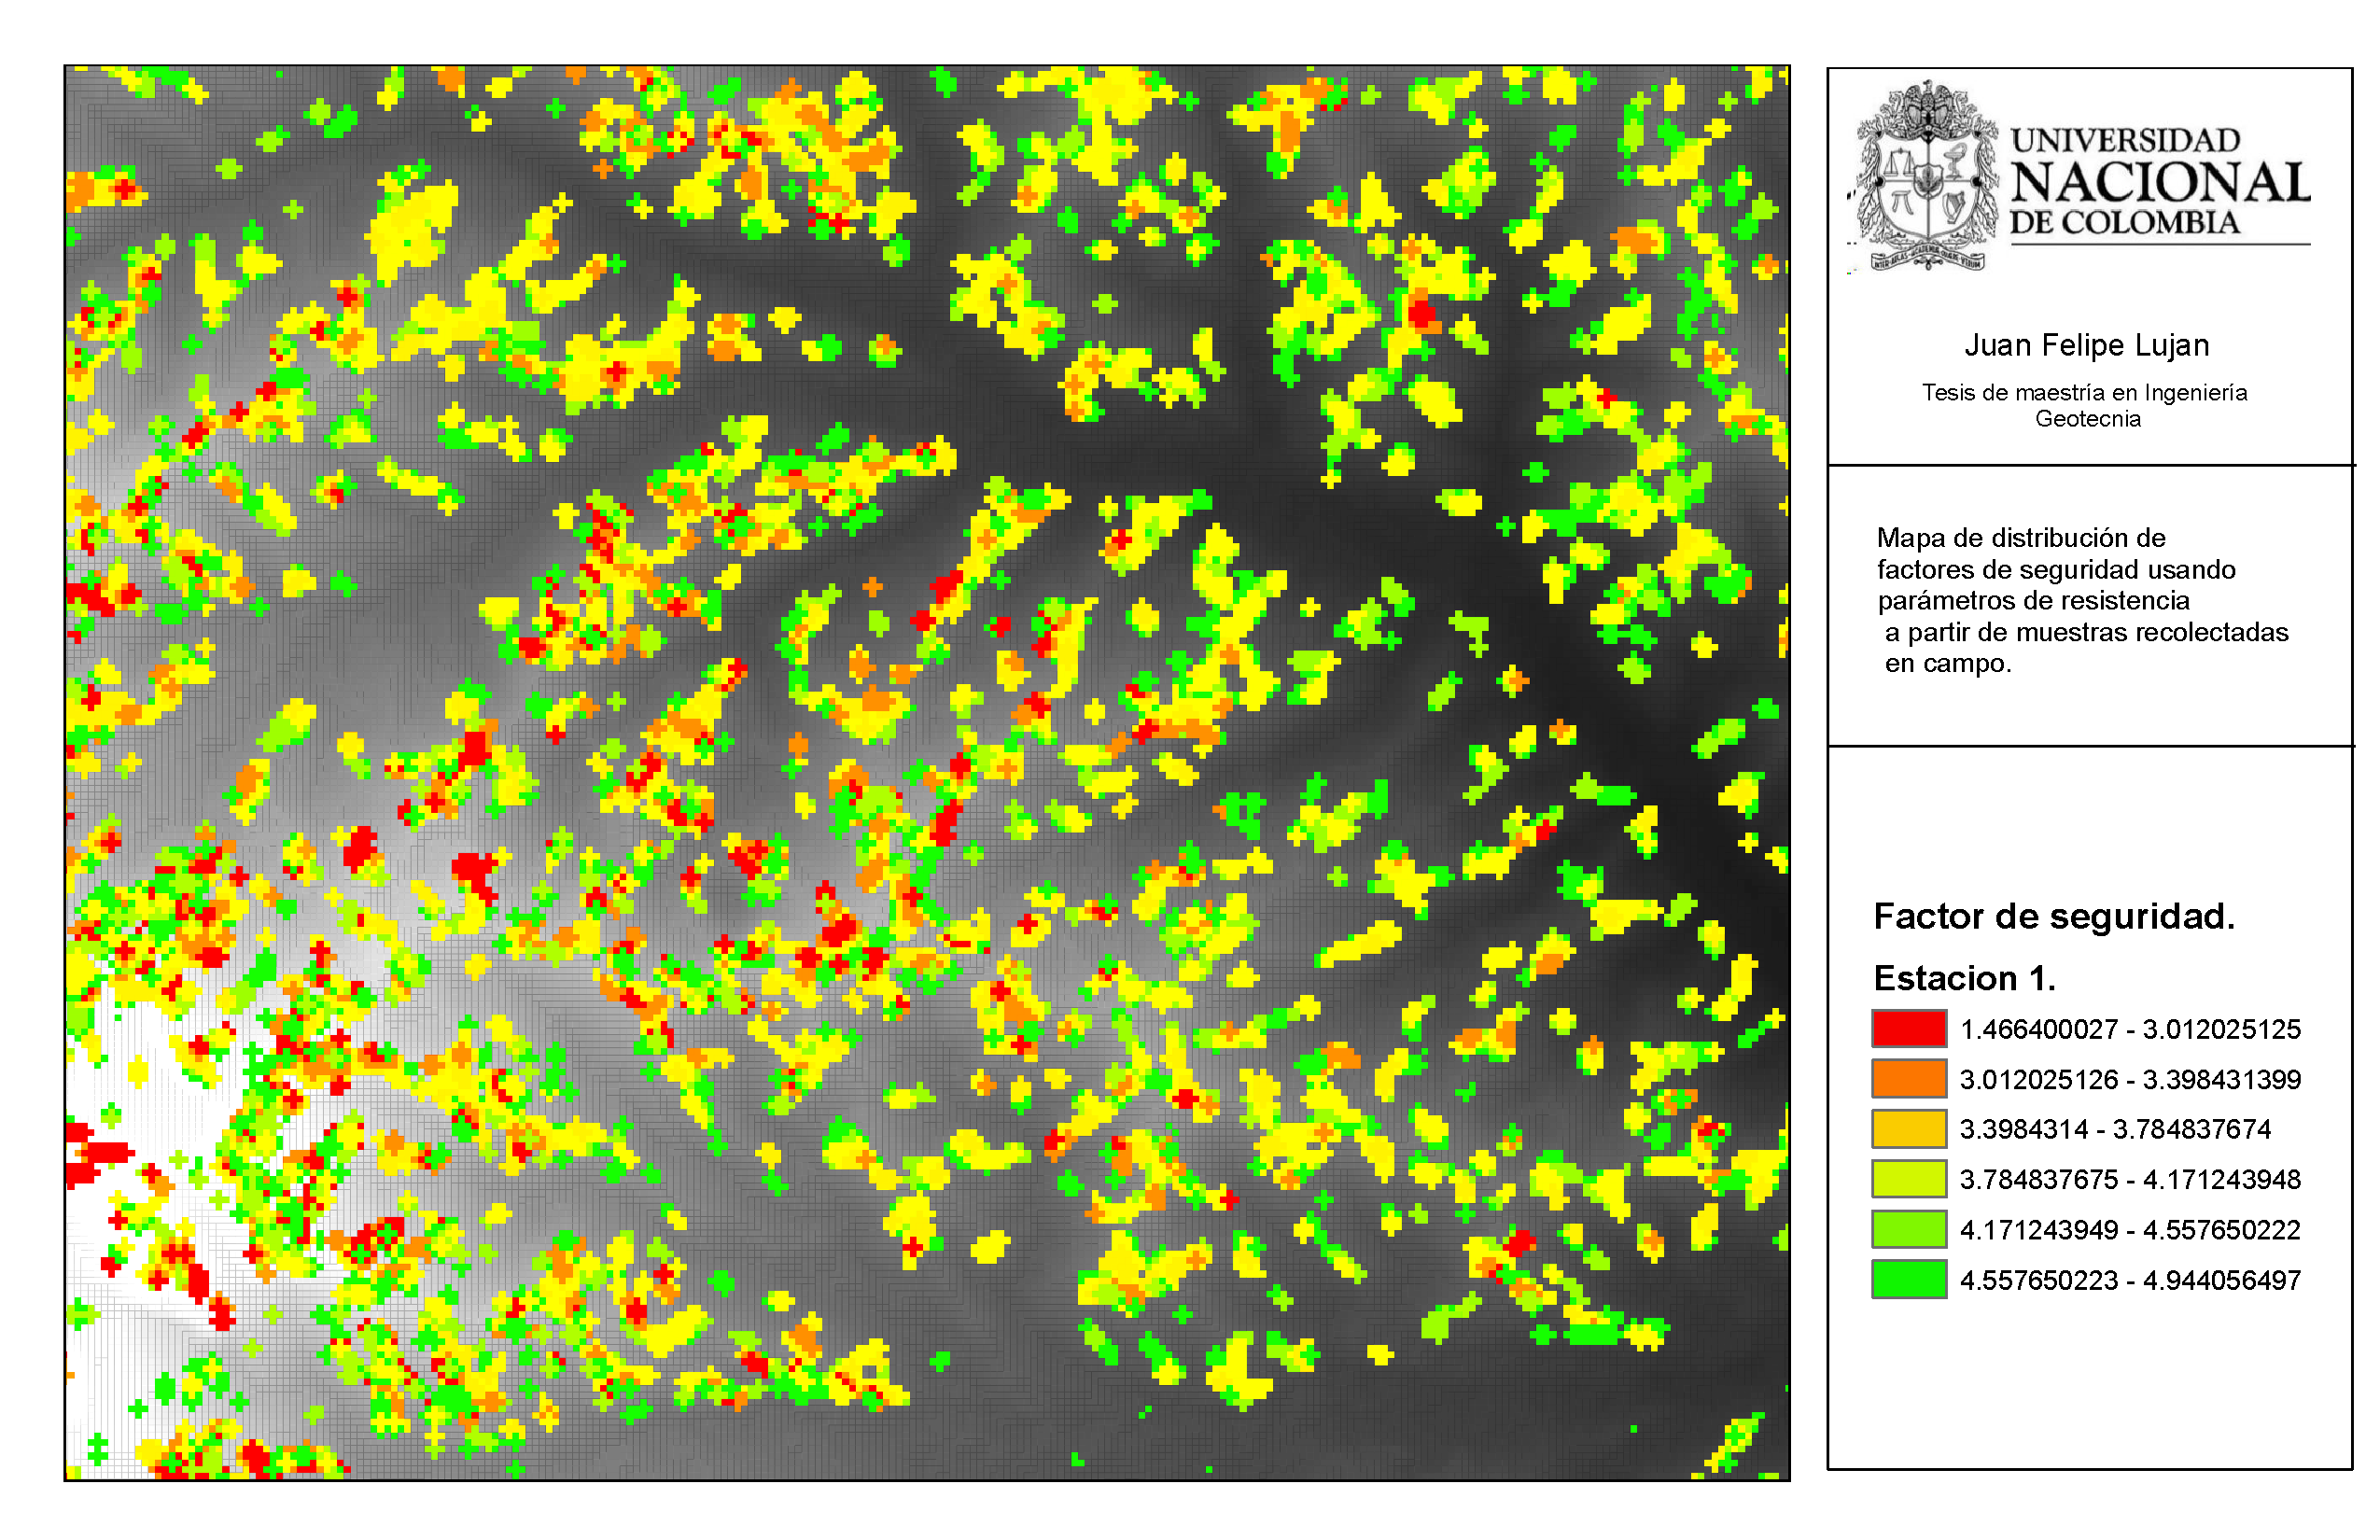
\includegraphics[scale=0.3]{img/fos3DCampo.pdf}
\caption{Mapa de distribuci�n de factores de seguridad en la zona de trabajo seg�n el an�lisis realizado con scoops 3D y muestras de la zona. Fuente: Elaboraci�n propia.}
\label{fig:fos3dout}
\end{figure}

Como resultado del analisis probabilistico por medio del metodo bishop utilizando las valores de resistencia obtenidos en los analisis de laboratorio realizadas a las muestras recolectadas del area de trabajo se obtiene el mapa de distribuciones de factores de seguridad presentado en la figura 6.2.
Se analizaron un total de 285744 superficies de falla

Como es de esperarse, los valores de factor de seguridad mas bajos se presentan hacia el suroccidente de la zona de trabajo, donde se son abundantes laderas con pendientes  largas y pronunciadas. All� los valores de factor de seguridad obtenidos de alcanzan 1.46 en cercanias al Batolito Farallones y su aureola de contacto.

Si se considera un cutoff de 3.0 para el factor de seguridad, el cuerpo de masa de mayores dimensiones con factor de seguridad  inferior a dicho cutoff (2.43 espec�ficamente) posee una masa de $9.544$ Kg, in volumen de $231.34m^{3}$ y se extiende sobre $23.63m^{2}$.



\section{Conclusiones}


Aunque se han encontrado zonas especificas con factor de seguridad bajo, estas abarcan extensiones bastante bajas y distribuidas, no se han detectado zonas de embergadura considerable con \textit{F} inferior a 3.0

La informaci�n de cohesion, �ngulo de fricci�n y peso especif�co tradicionalmente usado en bishop simplificado a 2 dimensiones puede usarse como insumo para extender el an�lisis  de equilibrio limite a 3D simensiones.

El uso de Scoops3D se ve altamente beneficiado por el uso de informaci�n SIG de alto nivel de detalle, toda vez que reduce la aparici�n de multiples subsets por esfera de b�squeda.



\section{Recomendaciones}

Previo al uso de la herramienta Scoops3D se recomienda en realizar un proceso de control de calidad sobre el DEM utilizado. Con el proposito de extraer los metadatos de extension horizontal y veltical del mismo para el momento de asignar las dimensiones a la caja de busqueda en Scoops3D

Seleccionar siempre la opcion de Bishop dentro del menu de seleccion de analysis de estabilidad, ya que esta opcion calcula el factor de seguridad tanto por Bishop simplificado como por el m�todo de Fellenius.
